%  This LaTeX template is based on T.J. Hitchman's work which is itself based on Dana Ernst's template.  
% 
% --------------------------------------------------------------
% Skip this stuff, and head down to where it says "Start here"
% --------------------------------------------------------------

\documentclass[12pt]{article}
\usepackage[margin=1in]{geometry} 
\usepackage{amsmath,amsthm,amssymb}
\usepackage{graphicx}
\usepackage{listings}
\usepackage{hyperref}
\usepackage[nottoc]{tocbibind}

\hypersetup{
	colorlinks=true,
	linkcolor=blue,
	filecolor=magenta,      
	urlcolor=cyan,
}
\newenvironment{statement}[2][Statement]{\begin{trivlist}
		\item[\hskip \labelsep {\bfseries #1}\hskip \labelsep {\bfseries #2.}]}{\end{trivlist}}
\begin{document} 
	\title{Midterm Progress Report}
	\author{Eric L. Lee, Yu-Cheng Weng, Can Jiang, Shu-Hao Chang} 
	\maketitle
	
	\section{Abstract}
	
	In our last proposal report, we planned to perform link prediction on network structured data.
	By now, we have collected data and established our evaluation framework. We implemented 6 baseline models in 8 different datasets, performed data analysis and visualized our datasets. In the following three weeks, we will be focusing on implementing factorization models and state-of-the-art methods as well as further improving our current results. 
	
	\section{How to Reproduce Our Result}
	We believe that reproducibility is very important when it comes to research. Thus, we carefully recorded all of our experiment results on Github. All the results presented in the following sections can be easily reproduced using this github repository: 
	\\
	\\
	\url{https://github.com/miamiasheep/Purdue\_ML\_Course\_Project}
	\\
	\\
	To reproduce all of our result (including data analysis part), simply type the following commands: 
	\begin{lstlisting}
	python script.py
	\end{lstlisting}
	To reproduce the result of certain data sets, type the following command:
	\begin{lstlisting}
	python main.py --input [file1,file2,...] --goal [auc/f1]
	\end{lstlisting}
	To draw the graph of a network, type the following command:
	\begin{lstlisting}
	python main.py --input [file] --draw [N(Integer)]
	\end{lstlisting}
	When N is larger, the sample network will be larger.
	
	\section{Data Analysis}
	
	\subsection {Data Set}
	We collect 8 different datasets which are all unique and have different characteristics. Table \ref{tab:info} shows basic statistics of each data set.
	\subsubsection{Facebook}
	This is a dataset downloaded from SNAP(Staford NEtwork Analysis Project)\cite{snapnets}. The data is an egonet in facebook. Each node represents an account in Facebook and each link represents friendship in Facebook.
	\subsubsection{Power}
	Power is  an electrical grid of western US\cite{small_world}.
	\subsubsection{NS}
	NS is a collaboration network of resarchers who publish paper on network sciences \cite{Newman_2006}.
	\subsubsection{PB}
	PB is a network of US political blogs.\cite{pb}
	\subsubsection{Router}
	Router is a router-level Internet.\cite{router}
	\subsubsection{USAir}
	USAir is a network of US air lines. \cite{usair}
	\subsubsection{Yeast}
	Yeast is a protein-protein interaction network in yeast.\cite{yeast}
	
	\subsubsection{Celegan}
	Celegan is a neural network of C. elegans.\cite{small_world}
	
	\begin{table}
		\begin{center}
			\begin{tabular}{|c|c|c|c|c|}
				\hline
				data set & nodes & edges & average degree & max degree \\
				Facebook & 4039 & 88234 & 21.85 & 1045 \\
				Power & 4941 & 6595 & 1.33 & 19 \\
				NS & 1461 & 2742 & 1.87 & 34 \\
				PB & 1222 & 16714 & 13.68 & 351 \\
				Router & 5022 & 6258 & 1.26 & 106 \\
				USAir & 332 & 2126 & 6.40 & 139 \\
				Yeast & 2375 & 11683 & 4.91 & 118 \\
				Arxiv & 18772 & 198110 & 10.55 & 504 \\
				Celegan & 297 & 2148 & 7.23 & 134 \\
				\hline 
			\end{tabular}
			\caption{Basic Information of different data set}
			\label{tab:info}
		\end{center}
	\end{table}
	
	\subsection{Visualizing Our Data Set}
	We implemented a tool to visualize our datasets. And all of our visualization graphs can be seen in the following link:
	\\
	\\
	\url{https://github.com/miamiasheep/Purdue_ML_Course_Project/tree/master/graph}
	\\
	\\
	Since the network is too big and it is hard to find any clue regarding the network structure if we draw all the edges and nodes, we only sampled a small portion of the network on every dataset.
	\\
	\\
	By visualizing our data sets, we can see that the characteristic of each data is actually very different. Let's take Facebook (figure\ref{fig:facebook}) and Router (figure\ref{fig:Router}) as examples. Facebook dataset has multiple triangles in the middle of the network. In contrast, Router has no triangle in the data set.
	
	
	\begin{figure}[h]
		\centering
		\includegraphics[scale=0.3]{Facebook}
		\caption{facebook}
		\label{fig:facebook}
	\end{figure}
	
	\begin{figure}[h]
		\centering
		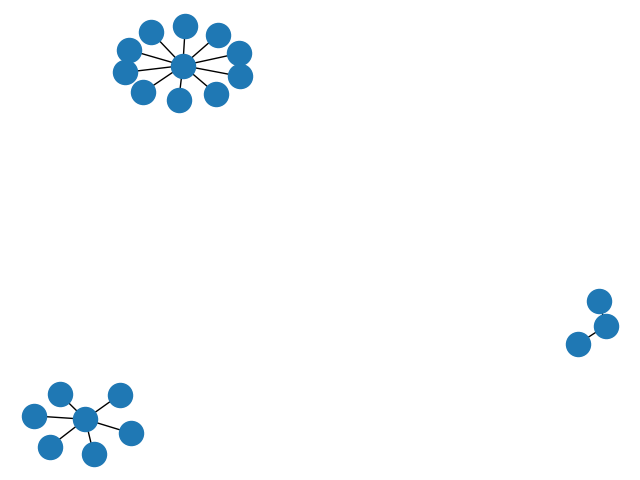
\includegraphics[scale=0.3]{Router}
		\caption{Router}
		\label{fig:Router}
	\end{figure}
	\section{Evaluation and Result}
	
	\subsection{Baselines}
	For the following sections, we denote x and y as two nodes, between which we want to predict if there is a link. And we denote the set of neighbors of x as N(x). We implemented six very common heuristics. And in \ref{tab:method}, we organized the formulas of the six heuristics. \\
	\subsubsection{Common Neighbors(CN)}
	It is a very simple heuristic. The intuition is that the more common neighbors the two nodes have, the more likely that there is a link between them. The score can be calculated as $|N(x) \cap N(y)|$.
	\subsubsection{Jaccard(JC)}
	It is very similar to common neighbors except that Jaccard considers the fact that two higher degree nodes unsurprisingly tend to have more common nodes. Thus, if two lower degree nodes have common neighbors, maybe they really have a strong relationship. The score can be calculated as $\frac{|N(x) \cap N(y)|}{|N(x) \cup N(y)|}$
	\subsubsection{Adamic Adar(AA)}
	It is also very similar to common neighbors. It assumes that a low degree common neighbor have more contribution to the probability of a link between x and y. Thus, the score divides the weight of each common neighbor by the logarithm of its degree. It is actually very similar to TFIDF. And we can calculate the Adamic Adar by $\sum_{z \in N(x) \cap N(y)}{\frac{1}{log(|N(z)|)}}$
	\subsubsection{Total Neighbors(TN)}
	It is the simplest baseline, which is just summing up the total size of neighbors of x and y. It can be calculated as $|N(x)| + |N(y)|$
	\subsubsection{Preferential Attachment(PA)}
	It is assumed that a high degree node have more chances to have a link with other nodes. Preferential Attachment calculate the product of degree of x and y. It can be calculated as $|N(x)| * |N(y)|$
	\subsubsection{Page Rank(PG)}
	It is very similar to PA. But instead of using the product of nodes' degrees, it uses the product of two nodes' scores derived from performing page rank on our network. Since the product can be very small, we use the sum of logarithm instead. Let $r_x$ be the score of x after performing page rank and $r_y$ be the score of y after page rank. It can be calculated as $\log{r_x} + \log{r_y}$
	\begin{table}
		\begin{center}
			\begin{tabular}{|c|c|}
				\hline
				method & description \\
				\hline
				common neighbor(CN) & $|N(x) \cap N(y)|$ \\
				Jaccard(JC) & $\frac{|N(x) \cap N(y)|}{|N(x) \cup N(y)|}$ \\
				Adamic and Adar(AA) & $\sum_{z \in N(x) \cap N(y)}{\frac{1}{log(|N(z)|)}}$ \\
				Total Neighbor(TN) & $|N(x)| + |N(y)|$ \\
				Preferentail Attachment (PA) & $|N(x)| * |N(y)|$ \\
				Page Rank(PR)  & $\log{r_x} + \log{r_y}$ \\	
				\hline
			\end{tabular}
		\end{center}
		\caption{link prediction methods}
		\label{tab:method}
	\end{table}
	
	\subsection{Evaluation}
	Evaluation is not trivial when it comes to link prediction problems. If we want to evaluate all pairs of nodes, it will take O($N^2$) prediction time, where N is the size of the nodes. And even for a small graph with 1000 nodes, the evaluation time is a lot. In fact, finding a fair and effective evaluation is also a research topic. Ryan and Nitech published a paper about how to evaluate a link prediction problem. We choose the most common way to evaluate our model: Down-sampling negative samples. (By negative samples, we mean a pair of nodes with no link between them. In link prediction problems, negative samples are usually way more than positive ones.)
	\\
	\\
	First, we randomly divided our edges into training, validation and testing. The ratio is 0.8:0.1:0.1. Training set is for training while validation set is only for grid search for the best parameters. And testing set is for evaluation of our model. 
	\\
	\\
	Second, we randomly sampled negative samples for validation and testing set. The sample size is equal to the set size.
	\\
	\\
	Third, we trained the models, applied the models to our testing set, and ranked the pairs by their scores. The higher score a pair gets, the higher the ranking it is and the more possible that there would be a link between them. For evaluation, we then used the ranking metrics. We mainly used AUC-ROC score (area under Receiver Operating Characteristics curve, abbreviated to AUC here). AUC has a very good characteristic that the sampling AUC is actually an approximation of actual AUC even if we do down-sampling. However, in real applications, even if our models give high rankings for the positive samples in the testing set, it's likely that they might not be ranked high in the real dataset because there are much more negative samples in reality. Therefore, we also implemented f1@k score as an evaluation metric. For the parameter k, we tentatively set the k equal to the size of positive samples. For this k, recall is actually equal to precision. And f1@k thus has a very intuitive physical meaning: the accuracy of finding all of the missing links given the size of missing links. In the future, we'll try to set different k's and see the influence of them. 
	\\
	\\
	Also, something to note here is that some nodes may only exist in validation or testing set but not in training set. We discarded the pairs of nodes where at least one node is not in the training set when evaluating, i.e., We only considered pairs of which both nodes are in the training set.
	
	
	\section{Result and Discussion}
	\begin{table}
		\begin{center}
			\begin{tabular}{|c|c|c|c|c|c|c|}
				\hline
				Data Set & CN & JAC & AA & PA  & TN & PG \\
				\hline
				Celegans&0.8314&0.7669&0.8443&0.7554&0.734&0.7998\\
				facebook&0.9882&0.9863&0.9893&0.8324&0.7345&0.8198\\
				NS&0.9742&0.9747&0.9741&0.6803&0.5204&0.7062\\
				PB&0.9152&0.8669&0.9176&0.908&0.8776&0.9175\\
				Power&0.5965&0.5964&0.5965&0.528&0.5198&0.7757\\
				Router&0.6109&0.6102&0.6111&0.9298&0.9198&0.9659\\
				USAir&0.9509&0.9164&0.9626&0.9021&0.868&0.9188\\
				Yeast&0.902&0.901&0.9029&0.8561&0.7926&0.8864\\
				\hline
			\end{tabular}
		\end{center}
		\caption{AUC of the six baselines}
		\label{tab:auc}
	\end{table}
	
	\begin{table}
		\begin{center}
			\begin{tabular}{|c|c|c|c|c|c|c|}
				\hline
				Data Set & CN & JAC & AA & PA & TN & PG \\
				\hline
				Celegans&0.7407&0.5926&0.713&0.5694&0.5787&0.6296\\
				facebook&0.9546&0.9312&0.9544&0.6742&0.5618&0.655\\
				NS&0.9524&0.9524&0.9524&0.5281&0.3939&0.4935\\
				PB&0.8052&0.6927&0.801&0.7762&0.7223&0.7846\\
				Power&0.1947&0.1947&0.1947&0.396&0.3518&0.5199\\
				Router&0.2279&0.2279&0.2279&0.761&0.7574&0.8272\\
				USAir&0.8278&0.7608&0.8612&0.799&0.7799&0.7608\\
				Yeast&0.815&0.815&0.815&0.7024&0.6184&0.7274\\
				\hline
			\end{tabular}
		\end{center}
		\caption{F1 score of the six baselines}
		\label{tab:f1}
	\end{table}
	
	Table \ref{tab:auc} shows AUC's of the six different baselines and Table \ref{tab:f1} shows the F1 scores.
	\\
	\\
	According to the result above, we can see that no heuristic method can outperform all other heuristics, and that Adamic Adar(AA), Jaccard, and common neighbors perform pretty well in the Facebook and NS dataset. However, for Power and Router dataset, the results of common neighbor based methods are pretty bad. This is not surprising because in Power and Router dataset, there are so few triangles that the methods aren't able to achieve good performances. 
	
	\section{Future Work}
	We will keep working on what we have proposed in our proposal. Since we have finished our evaluation framework, we can start implementing our machine learning models. And the final results will be included in our final report. 
	
	
	
	\bibliographystyle{acm}
	\bibliography{midterm_progress_report}
	
	
\end{document}